\vsp
\section{ \auspice\ design \& implementation}
\label{sec:design}

%In this section, we present \auspice, a massively scalable global record service designed for high mobility. We begin by describing how the envisioned service enables endpoint mobility, and the requirements in order to realize that vision.


\subsection{Design goals}
\label{sec:design_goals}

Our goal is to design a distributed system that meets the following requirements:

{\bf (1) Low lookup latency}: Replicas of a key should be placed close to end-users accessing it so as to minimize user-perceived response times.


%An implicit goal here is to not only support use-cases like above but also to enable other architectural proposals that involve routers late-binding records to addresses near the destination \cite{serval,MobilityFirst-UMASS}; enabling seamless mid-connection mobility \cite{Migrate,ECCP}, etc., so that any endpoint or router gets the feel of the lookup service being located tens of milliseconds away.

{\bf (2) Resource cost}: The design must ensure low replication cost. A naive way to minimize lookup latencies is to replicate every record at every possible location, however high mobility means high update rates, so the cost of pushing each update to every replica would be prohibitive. Worse, load hotspots can actually degrade lookup latencies.

{\bf (3) High availability}: The design must ensure resilience to node failures including outages of entire datacenters; by consequence, it should also prevent crippling load hotspots.

{\bf (4) Consistency}: The design must provide flexible consistency semantics as desired by an application.

%Note that ``scalability'' is not an explicitly defined goal above because it is subsumed by the first three goals, i.e., a design maximizing performance and availability for any given resource cost is implicitly designed to improve the former with commensurately more resource expenditure. We explicitly quantify this tradeoff in $\S$\ref{sec:scalability}.


\subsection{\auspice's geo-distributed design}
\label{sec:design_overview}

To address the above goals, the \auspice\  is designed as a massively geo-distributed key-value store. The geo-distribution is essential to the latency and availability goals while the key-value API is chosen for its popularity among today's web services. Each {\em record} in \auspice\ is associated with a globally unique identifier (GUID) that is the record's primary key. A record contains an associative array of key-value pairs, wherein each key $K_i$ is a string and the value $V_i$ may be a string, a primitive type, or recursively a key-value pair, as shown below.

GUID  $\ | \ K_1, V_1 \ | \ K_2, V_2 \ \ | \cdots $

%By default, all columns and network addresses in particular can be read by all but written to only using the GUID's private key. Some {\em keyword} attributes like netAddress and geoLocation have special support (unlike developer-defined attributes), for example, in order to efficiently maintain indexes for value-based reverse lookups or for non-default privacy policies like allowing only whitelisted reads for geoLocation.

%For the former, it suffices to think of a {\em record} as a domain record, a {\em record} as the associated zone file, and a {\em server} as analogous to a DNS server. For ease of exposition, we assume one server per geo-location.

%\subsection{\auspice's geo-distributed design}

\begin{figure}[t]
\centering
\vspace{-0.3in}
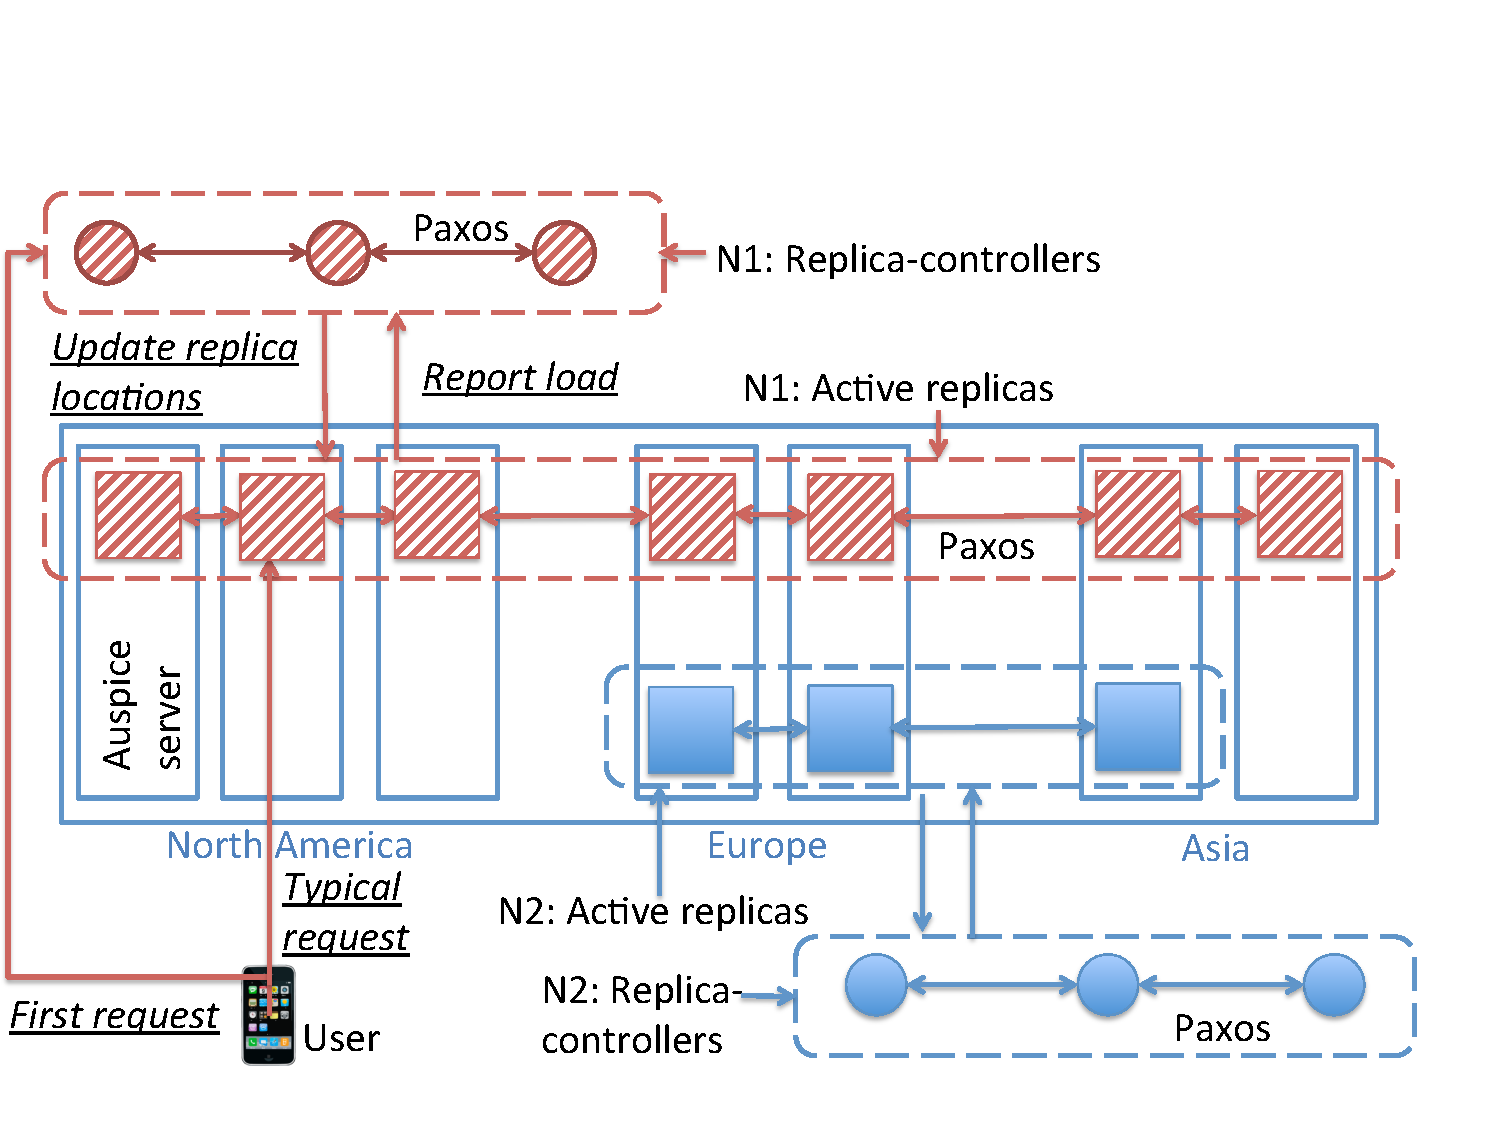
\includegraphics[scale=0.33]{gns-dns/gnrs.pdf}
\vspace{-0.35in}
\caption{Geo-distributed servers in \auspice.  Replica-controllers  (logically separate from active replicas) decide placement of active replicas and active replicas handle requests from end-users. N1 is a globally popular record and is replicated globally; record N2 is  popular in select regions and is replicated in those regions.}
\vspace{-0.2in}
\label{fig:auspice}
\end{figure}


At the core of \auspice\ is a placement engine that achieves the latency, cost, and availability goals by adapting the number and locations of replicas of each record in accordance with (1) the lookup and update request rates for the record, (2) the geo-distribution of requests for the record, and (3) the aggregate request load across all records. 

%The key to ensuring high availability and flexible consistency is a two-tier consensus engine for each record; the first ``control'' tier infrequently recomputes and migrates the current set of replicas of each record, and the second ``data'' tier upon each write or read coordinates with other replicas to ensure the necessary consistency semantics.% In addition to the placement algorithm, the design and implementation challenges we address include managing a very large number of parallel Paxos instances (one per record per tier); correctly changing Paxos group membership in a live system; efficiently routing client requests;  TBD\tbd{Need to say why challenging somewhere clearly}.


Figure \ref{fig:auspice} illustrates the placement engine. Each record is associated with a fixed number, $F$, of  \emph{replica-controllers} and a variable number of  {\em active replicas} of the corresponding record. The record's replica-controllers are computed using consistent hashing to select $F$ consecutive or otherwise deterministic nodes along the ring {\em onto} which the hash function maps records and nodes. The replica-controllers are responsible only for determining the number and locations of the active  replicas, and the actives replicas are responsible for maintaining the actual record and processing client requests. The replica-controllers implement a replicated state machine using Paxos \cite{LamportPaxos} in order to maintain a consistent view of the current set of active replicas.



%The key insight in \auspice\ is a placement engine to compute the number and locations of replicas of a record  based on the lookup to update ratio of the record,  the geo-distribution of its demand, and the aggregate request load on the system.

%
%At an abstract level, \auspice\ design can be described as consisting of two planes: a ``control plane'' which determines the locations at which each record is replicated, and a ``data plane''  consisting of  replicas of records whose function is to handle address lookups and updates for end-users.  Physically, both these planes run across the set of servers on which \auspice\ is deployed. 
%
%
%The role of the control plane for a record is handled by a fixed number, $M$, of  \emph{replica-controllers}. The number and locations of the replica-controllers is fixed and is computed using $M$ well-known consistent hash functions each of which maps the record to a server location. The replica-controllers implement a replicated state machine using Paxos \cite{LamportPaxos} so as to maintain a consistent view of the current set of active replicas despite failures. 
%

%The control plane periodically runs a placement algorithm and places a record based on the inferred pockets of demand for that record, the lookup-to-update ratio of the record, and the aggregate system load so as to achieve low lookup latency, low update cost, and desired level of availability. 



% achieve low response times, low update costs, and high availability.
%based on the geo-locality of demand for that record while mitigating load hotspots across all locations. 

%The key insight in \auspice\ is a placement engine to compute the number and locations of resolver replicas for a record based on the geo-locality of demand for that record while mitigating load hotspots across all locations. 

%% 'Active replicas' or  'replicas'?

%Figure \ref{fig:auspice} illustrates the architecture of \auspice.  Each record is associated with a fixed number, $M$, of  \emph{replica-controllers} and a variable number of  {\em active replicas} of the corresponding resolver. The locations of the replica-controllers is fixed and computed using $M$ well-known consistent hash functions each of which maps the record to a server location. The replica-controllers form the ``control plane'' and are responsible only for determining the number and locations of active replicas, and the active replicas are responsible for maintaining resource records and responding to lookup and update requests. 


%

A record's replica-controllers compute its active replica locations in a {\em demand-aware} manner. This computation proceeds in epochs as follows. At creation time, the active replicas are chosen to be physically at the same locations as the corresponding replica-controllers. In each epoch, the replica-controllers obtain from each active replica a summarized load report that contains the request rates for that record from different {regions} as seen by that replica. Here, {\em regions} partition users into non-overlapping groups that capture locality, e.g., IP prefixes or a geographic  partitioning based on cities; and the {\em load report} is a spatial vector of request rates as seen by the replica. The replica-controllers aggregate these load reports to obtain a concise spatial distribution of all requests for the record.



\eat{
The replica-controllers execute Paxos to compute the placement decision in a coordinated manner for each record. During periods of graceful execution, only one replica-controller (the Paxos coordinator) actually invokes the mapping algorithm while the others simply accept its proposed placement; consensus ensures that the replica-controllers maintain a consistent view of the current set of active replicas despite failures.
}

%\begin{figure}[t]
%\begin{center}
%%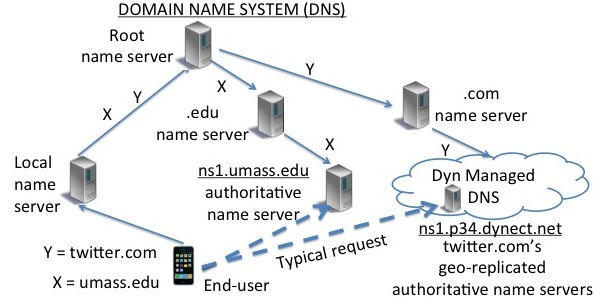
\includegraphics[width=3in, height=2.4in]{Auspice-arch/Slide1}
%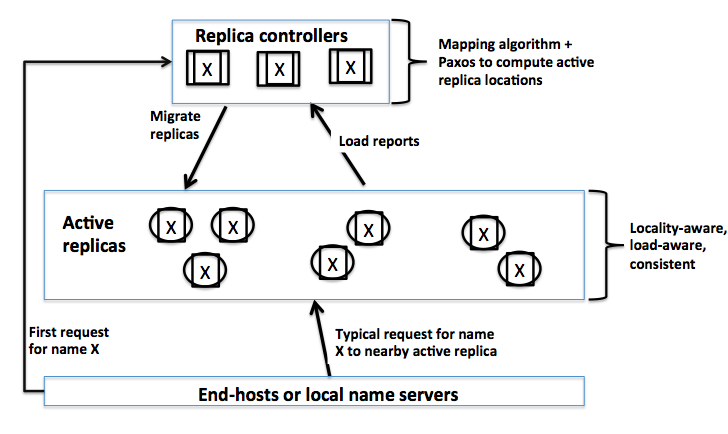
\includegraphics[width=3in]{graph/slide2SS}
%\vspace{-0.2in}
%\caption{\auspice\ design: Clients send typical requests to nearby active replicas of resolvers. Replica-controllers compute the number and locations of active replicas for each record based on load reports in each epoch.}
%\vspace{-0.2in}
%\label{fig:arch}
%\end{center}
%\end{figure}
\vsp
\subsubsection{Demand-aware replica placement} 
\label{sec:placement}

In each epoch, the replica-controllers use a {placement algorithm} that takes as input the aggregated load reports and capacity constraints at servers to determine the number and locations of active replicas for each record so as to minimize client-perceived latency. We have formalized this {\em global} optimization problem as a mixed-integer program and shown it to be computationally hard.  As our focus is on simple, practical algorithms, we defer the details of the optimization approach \cite{techreport}, using it only as a benchmark in small-scale experiments with \auspice's heuristic algorithm.

%We have shown that the placement problem can be formulated as a mixed-integer optimization problem that is computationally hard (refer to the tech report \cite{techreport}), so we use it only as a benchmark in small-scale experiments.

\auspice's placement algorithm is a simple heuristic  and can be run {\em locally} by each replica-controller. The placement algorithm computes the number of replicas using the lookup-to-update ratio of a record in order to limit the update cost to within a small factor of the lookup cost. The number of replicas is always kept more than the minimum number needed to meet the availability objective under failures.   The location of these replicas are decided to minimize lookup latency by placing a fraction of replicas close to pockets of high demand for that record while placing the rest randomly so as to balance the potentially conflicting goals of reducing latency and balancing load among servers.
%The location of these replicas are decided partly based on the locality of demand, while the rest of the replicas are placed randomly in order to achieve a good tradeoff between locality-awareness and load-balance. 



Specifically, the placement algorithm computes the number of replicas for a record as ($F+ \beta r_i/w_i$), where $r_i$ and $w_i$ are the lookup and update rates of record $i$; $F$ is the minimum number of replicas needed to meet the availability goal (\S \ref{sec:design_goals}); and $\beta$ is a replication control parameter that is automatically determined by the system so as to trade off latency benefits of replication against update costs given capacity constraints as follows. In each epoch, the replica-controllers recompute $\beta$ so that the aggregate load in the system corresponds to a preset threshold utilization fraction $\mu$. For simplicity of exposition, suppose read and write operations impose the same load, and the total capacity across all servers (in reads/sec) is $C$. Then, $\beta$ is set so that  
\vsp
\begin{equation}
\mu C = \sum_i r_i  + \sum_i (F + \beta  \frac{r_i}{w_i}) w_i
\label{eq:mu}
\end{equation}
\vsp
\vsp

 where the right hand side represents the total load summed across all records. The first term in the summation above is the total read load and the second is the total write load. 
%\begin{equation}
%\beta = \frac{C\mu - M \sum_i W_i}{\sum_i R_i}- 1
%\label{eq:beta}
%\end{equation}
%It is straightforward to extend the above heuristic to scenarios where read and write operations impose unequal amounts of load on a server
 
Having computed $\beta$ as above, replica-controllers compute the locations of active replicas for record $i$ as follows. Out of the $F + \beta r_i/w_i$ total replicas, a fraction $\nu$ of replicas are chosen based on locality, i.e., replica-controllers use the spatial vector of load reports to select $\nu(F + \beta r_i/w_i)$ servers that are respectively the {closest} to the top $\nu(F + \beta r_i/w_i)$ regions sorted by demand for record $i$. The remaining $(1-\nu)(F + \beta r_i/w_i)$  are chosen randomly without repetition. The locality-based replicas above are chosen as the {\em closest} with respect to round-trip latency plus load-induced latency measured locally at each server. An earlier design chose them based on round-trip latency alone, but we found that adding load-induced latencies in this step (in addition to choosing the remaining replicas randomly) ensures better load balance and lowers overall client-perceived latency.
Our current prototype and system experiments fix the random perturbation knob $\nu$ to 0.5. We have since developed a slightly modified placement scheme that relieves the administrator from setting $\nu$ manually, automatically balancing locality-awareness and load to ensure low latencies \cite{techreport}. Thus, an administrator need only specify F and $\mu$ based on fault tolerance and aggressiveness of capacity utilization.

\auspice's replica placement scheme (Eq. \ref{eq:mu}) is designed to use a fraction $\mu$ of system-wide resources so as to make at least $F$ and at most $M$ replicas of each record, where $M$ is the total number of server locations. Thus, at light load, \auspice\ may replicate every record at every location, while under heavy load, it may create exactly $F$ replicas for all but the most popular records. 


\subsubsection{Client request routing}
\label{sec:routing_client_requests}
A client request is routed from an end-host to a suitable server as follows. 
The set of all servers in an \auspice\ instance is known to each member server and can be obtained from a well-known location. 
When a client encounters a request for a record for the first time, it uses the known set of all servers and consistent hashing to determine the replica-controllers for that record and sends the request to the closest replica-controller. The replica-controller returns the set of active replicas for the record and the client resends the request to the closest active replica.  In practice, we expect replica-controllers to be contacted infrequently as the set of active replicas can be cached and reused until they change in some future epoch. %, and active replicas change across epochs only if the geo-locality of demand for the record changes significantly.
%client requests up to three active replicas to get a response.  A timeout value is set for every request sent and the request is sent to the next closest active replica on a timeout.

%To answer lookup requests, clients implement a TTL-based cache to store the records received.






%A client redirects end-users requests to a resolver chosen in a locality and load-aware manner. To achieve both these properties, clients maintain latency estimates to servers that reflect both network latency and server-load induced latency (or server latency). Among a set of resolvers,  a client always redirects requests to the closest server based on  the latency estimates. 

%A client in \auspice\ redirects end-users requests to a resolver chosen in a locality and load-aware manner. To achieve both these properties, clients maintain latency estimates to servers that reflect both network latency and server-load induced latency (or server latency). Among a set of resolvers,  a client always redirects requests to the closest server based on  the latency estimates.  Network latency estimates change slowly and therefore every client maintains round-trip latency estimates to all servers using infrequent measurements. Server latency changes frequently due to dynamic workloads.  In an Internet scale deployment with tens of thousands of servers, maintaining server latency information would add significant overhead.  Hence, server latency  is maintained only for a smaller number of frequently contacted servers.

Network latency as well as server-load-induced latency help determine the closest replica at a client. Each client maintains an estimate of the round-trip latency to all servers using infrequent pings; an (as yet unimplemented) optimization to reduce the overhead of all-to-all pings is to use coordinate embedding, geo-IP, or measurement-driven techniques \cite{iplane}. To incorporate load-induced latency, the latency estimate to a server is passively measured as a moving average over lookups sent to that server. The client also maintains a timeout value based on the moving average and variance of the estimates.  If a lookup request sent to a server times out, the client infers that either the server or network route is congested, and it multiplicatively increases its latency estimate to that server by a fixed factor. Thus,  if multiple lookups sent to a server time out, the estimated latency shoots up and the client stops sending requests to that  server, which effectively acts as a more agile load-balancing policy in the request routing plane (complementing the replica placement plane above that operates in coarser-grained epochs).


\subsubsection{Consistency with static replication}
\label{sec:consistency}

%\tbd{Rewrite entire section.}

%The above proximity-based strategy can route both lookup (or read) and update (or write) requests for a record to any active replica. In order to ensure low lookup latency, it is important for them to be served locally from an active replica. This means that the onus of replica coordination in order to maintain any nontrivial consistency semantics falls on the update procedure. But why should we care about consistency when DNS and network protocols in general prize liveness over consistency\cite{consensus-routing}?

As a geo-distributed key-value store, \auspice\ must at least ensure this eventual consistency property: {\em all active replicas must eventually return the same value of the record and, in a single-writer scenario, this value must be the last update made by the (only) client}; ``eventually" means that there are no updates to a record and no replica failures for sufficiently long. Violating this property means that a client may be  indefinitely unable to obtain the the up-to-date value of the record even though the record is no longer being updated. 

With a static set of replicas, it is straightforward to support this property. A replica receiving  a client update need only record the write in a persistent manner locally, return a commit to the client, and lazily propagate the update to other active replicas for that record. Lazy propagation is sufficient to ensure that all replicas eventually receive every update committed at any replica, and a deterministic reconciliation policy, e.g., as in Dynamo \cite{dynamo}, suffices to ensure that concurrent updates are consistently applied across all replicas. Temporary divergence across replicas under failures can be shortened by increasing durability, i.e., by recording the update persistently at more replicas before returning a commit to the client. The additional ``single-writer" clause is satisfied simply by incorporating a client-local timestamp in the deterministic reconciliation policy. 

%It would appear that this weak eventual consistency property can be easily satisfied if the client associates a sequence number with each update; an active replica can simply locally record the write, return to the client, and lazily propagate the update to other active replicas.

%Unfortunately, the simplistic approach above has some problems. As the set of active replicas for a record can change over time, a write-to-one approach can lose the most recent write if the active replica that received the write crashes and before it recovers, the replica controllers change the set of active replicas. Even if the set of active replicas remains unchanged, the window of inconsistency (or unreachability) is higher with a write-to-one approach if the active replica that received the write fails. Most importantly, we anticipate that expressive records (see $\S$\ref{sec:extsec}) may be updated by multiple authorized clients via different active replicas, and it is important to ensure that update operations (like appending to or deleting from a list) to a record are applied in the same order by all active replicas. These requirements motivate a state-machine approach to handle updates. 

\textbf{Total ordering.} To be useful to a broader set of applications that demand more sophisticated query patterns, it may be useful in some scenarios to ensure that update operations (like appending to or deleting from a list) to a record are applied in the same order by all active replicas. Ensuring a total ordering of all updates to a record is a stronger property than eventual consistency, calling for a state-machine approach, which \auspice\ supports as an option. In fact, \auspice\ supports an option to perform total ordering of all updates and lookups as well, which is a even stronger property than total write ordering alone.


To this end, active replicas for a record participate in a Paxos instance maintained separately for each record (distinct from Paxos used by replica-controllers to compute active replicas for that record). Each update is forwarded to the active replica that is elected as the Paxos coordinator that, under graceful execution, first gets a majority of replicas to accept the update number and then broadcasts a commit. Total write ordering of course implies that updates can make progress  only when a majority of active replicas can communicate with each other while maintaining safety (consistent with the so-called CAP dilemma).

\vsp
\subsubsection{Consistency with replica reconfiguration}
\label{sec:reconfiguration}

With a dynamic set of replicas as in \auspice, achieving eventual consistency is straightforward, as it suffices if a replica recovering from a crash lazily propagates all pending writes to a record to its {\em current} set of active replicas as obtained from any of the consistently-hashed replica-controllers for the record. However, satisfying the (optional) total write order property above is nontrivial.

To this end, we have designed a two-tier reconfigurable Paxos system that involves explicit coordination between the consensus engines of the replica-controllers and active replicas. Reconfiguration is accomplished by a replica-controller issuing and committing a stop request 
%\cite{lamport2008stoppable} 
that gets committed as the last update of the current active replica group. The replica-controller subsequently initiates the next group of active replicas that can obtain the current record value from any member of the previous group. This design shares similarities with Vertical Paxos \cite{vertical-paxos}, however we were unable to find existing implementations or even reference systems using similar schemes, so we had to develop it from scratch. The details of the reconfiguration protocol are here \cite{techreport}.


\subsubsection{Replica reconfiguration policies}
\label{sec:reconf_policy}

\blue{
The policy decision of when to reconfigure the replica group for a specific record is orthogonal to the consistency mechanisms above. The frequency of reconfiguration presents a tradeoff between agility to demand and the reconfiguration messaging overhead. This overhead includes (1) load reports per epoch from active replicas to replica-controllers; (2) replica-controllers computing the new set of active replicas by consensus; (3) replica-controllers notifying the old active replicas to stop and the new ones to start; and (4) newly added replicas obtaining the record state from any old replica, and (5) replica-controllers agreeing that the group change is complete. Each of these steps entails one or two small messages per record at each active replica or replica controller, except for step 4 where the overhead depends on the size of the record. The first overhead is incurred per epoch and can be further reduced by having an active replica issue a load report for a record only if the geo-locality of demand for the record has changed beyond a threshold at that replica. The subsequent steps are needed only if the policy deems reconfiguration as warranted based on the record's aggregate load report (noting that only a subset of records may need reconfiguration in an epoch).
}

\blue{
Thus, any reconfiguration policy that (1) limits load reports at an active replica to at most once per $m$ client requests for the record at that replica, and (2) limits reconfiguration at replica-controllers to at most once per $k m$ total client requests across the $k$ currently active replicas, suffices to ensure that the reconfiguration overhead is at most a fraction $\approx 1/m$ of the incoming client request load. As a consequence, it may take at least $m$ requests for a record at a new location before an active replica for it is created there.
}


\eat{
\subsubsection{Scalability: A performance-cost analysis}
\label{sec:scalability}

\blue{
{\bf{Cost}.} \auspice's replica placement scheme (Eq. \ref{eq:mu}) is designed to use a fraction $\mu$ of system-wide resources so as to make at least $F$ and at most $M$ replicas of each record, where $M$ is the total number of server locations. Thus, at light load, \auspice\ may replicate every record at every location, while under heavy load, it may create exactly $F$ replicas for all but the most popular records. In the common case, a lookup involves one request and response between a client and an active replica; an update involves $\approx$ thrice (twice) as many messages as the number of active replicas with total write ordering (eventual) consistency.
}

\newcommand{\ttc}{\textit{\sc{ttc}}}

\blue{
{\bf{Performance}.} The worst-case time-to-connect latency for a record $i$ depends on the lookup latency $l_i$, the update rate $w_i$, the worst-case update propagation latency $d_i$, i.e., the time for all active replicas to receive an update, and the connect timeout $T$, as follows \cite{techreport}.
\vsp
\begin{equation}
\ttc_i \ \ = \ \  l_i [1 + (e^{w_i d_i} - 1)(1 + \frac{T}{l_i})]
\label{eq:ttc}
\vsp
\end{equation}
}

\blue{
Thus, the time-to-connect increases with (1) the lookup latency $l_i$ that in turn improves with demand-aware replication; (2) the update rate $w_i$ and update propagation delay $d_i$ that in combination determine the likelihood of obtaining a stale response, noting that the latter increases with more aggressive replication; and (3) the connect timeout $T$ that is at most the default transport-layer timeout (e.g., a few seconds for TCP) and potentially as low as the round-trip delay between the connecting client and the destination being connected to if the destination network is capable of generating an ``no route to host'' error message.
}
\newcommand{\ttl}{\textit{\sc{ttl}}}

\blue{
{\bf{TTLs}.} The above analysis implicitly assumes near-zero TTLs. With a nonzero $\ttl_i$ for record $i$, the worst-case time-to-connect can be approximated as \cite{techreport}.
\vsp
\begin{equation}
\begin{split}
\ttc_i \ \ \simeq \ \ &\ \tau_i\  \frac{(r_i + w_i +  1/\ttl_i + r_i w_i \ttl_i)}{(1 + r_i \ttl_i)(r_i + w_i + 1/\ttl_i)} \\
& + \frac{T\ r_i \ w_i}{(r_i + 1/\ttl_i)(r_i + w_i + 1/\ttl_i)}
\end{split}
\vsp
\end{equation}
where $\tau_i$ above is $\ttc_i$ (with a 0 TTL) as in Eq \ref{eq:ttc}.
Thus, a long TTL is meaningful only if the update rate $w_i$ is low; if so, a carefully chosen TTL can reduce the load on the system as well as the client-perceived time-to-connect; if not, a long TTL can inflate the time-to-connect by the connect timeout $T$ ( = the second term above for $w_i\gg r_i$ and high $\ttl_i$).
}

%\begin{equation}
%\begin{split}
%\ttc_i \ \ = \ \ &\ l_i [1 + (e^{w_i d_i} - 1)(1 + \frac{T}{l_i})]\  \frac{(r_i + w_i +  1/\ttl_i + r_i w_i \ttl_i)}{(1 + r_i \ttl_i)(r_i + w_i + 1/\ttl_i)} \\
%& + \frac{T\ r_i \ w_i}{(r_i + 1/\ttl_i)(r_i + w_i + 1/\ttl_i)}
%\end{split}
%\vsp
%\end{equation}


\blue{
{\bf{Comparison to DNS}.} All of the above analyses are applicable also to geo-replicated managed DNS providers were they to employ \auspice's demand-aware replication approach. The main difference between \auspice\ and today's managed DNS providers that rely on simplistic static replica placement schemes is in the lookup latency $l_i$ achieved for any given resource cost; we evaluate this performance-cost tradeoff extensively in our experiments ($\S$\ref{sec:comparison} and $\S$\ref{sec:managed}). 
}
}


\eat {
As the group of active replicas can change over time, consistency guarantees depend on safely handling a change in the group of active replicas. The safety property can be stated as follows: {\em the group of active replicas in epoch $i+1$, before executing any requests, must obtain identical copies of the record and that copy must include all committed updates to the record made by the group of active replicas in epoch $i$}.

The key protocol for group change is Stoppable Paxos \cite{lamport2008stoppable}.   Stoppable Paxos supports a special STOP request that can be committed only once and is always the last request committed by the Paxos instance. The commit of the STOP request ensures that no further changes to the record will be made by the current group of active replicas. The next group of active replicas, before executing any requests, copy the  record from any of the current active replicas that have committed the STOP request.  This guarantees that each member in next group of active replicas starts with an identical copy of the record. Thus,  STOP acts as a link between the two otherwise independent Paxos instances per record: maintained by replica-controllers and active replicas respectively.
}

% write something about how replica controllers ensure that at most one change in the set of active replicas is in progress.



 
%the response of lookup requests sent by a client (irrespective of which replica the client sent a lookup to) always sees a monotonically increasing state of Paxos.

%
% If the response of a to the previous lookup request was returned by a replica with the state of a Paxos instance as 
%
% If the response to the previous lookup request was returned by a replica with the state of a Paxos instance as 
%   done when the state of the Paxos instance for the record was $s$, the next lookup is done with the state of Paxos instance at state $s1 \geq s$.
%
% If the previous lookup request was done when the state of the Paxos instance for the record was $s$, the next lookup is done with the state of Paxos instance at state $s1 \geq s$.
%
% and sees a result which is 
% responses to lookup requests for a record 
%received by a clients are in a monotonically increasing order in which they were committed.
% committing all update requests 
% by establishing a total order across all updates  for that record. A lookup request is processed locally at a replica. 
%
%\auspice\ ensures sequential consistency for address lookup/update operations for each record by establishing a total order across all updates of addresses for that record. This is achieved efficiently through Paxos\footnote{This per-write Paxos is distinct from  Paxos invoked by replica-controllers for computing the set of active replicas.} between active replicas upon a write. When an active replica receives a write to an record's address, it forwards the write to an active replica designated as the current Paxos coordinator. The coordinator selects a sequence number and sends an accept request to all replicas and, upon receiving a successful acknowledgment from a majority of replicas, sends a commit notification to all replicas. Thus, a typical write  request incurs four network delays (or two round-trips) to get committed after arriving at an active replica. A read request is processed locally at a replica and sees the result of the most recent committed write at that replica. 
%
%
%To maintain consistency in spite of a changing set of active replicas, Auspice uses the stoppable Paxos protocol \cite{lamport2008stoppable} among active replicas.  A Paxos instance running this protocol can be safely shut down after a special STOP command is committed; the STOP command is committed only once and is the last command committed by the Paxos instance. When the set of active replicas is to be changed, the Paxos instance among currently active replicas is shut down, the new active replicas copy the record from any of the previous active replicas, and a new Paxos instance is started among the new set of active replicas. The commands to stop (start) the Paxos instance between the old active replicas  (new active replicas) are sent by one of the replica-controllers.
%


%Further, we  describe how \auspice\ changes the set of active replicas, and handles server failures. 

%Active replicas for a record keep an entry for the record in persistent storage. This entry is called a \emph{record}.  Active replicas for a record form a Paxos instance, which  determines the order of all writes to the record at active replicas.  Replica-controllers for a record, like active replicas, keep an entry for the record, called a \emph{replica-controller record}, in persistent storage.  Replica-controllers for a record form a Paxos instance (separate from Paxos between active replicas), which  determines the order of all writes to the replica-controller record.

% that the  record has been deleted by replica-controllers, the replica-controllers have agreed that the record is to deleted but the deletion is in progress,  is going to be deleted, or is in neither of the two states.

%Replica-controller record does not contain the network addresses for a record.



%maintain a record known as the \emph{record}. 

%\auspice\ maintains two types of records for each record: (1) \emph{record} stored at active replicas which (among other fields) contains the current network address for a record and (2)  \emph{Replica-controller record} stored at replica-controllers which contains (among other fields)  a three tuple for both the current set and the previous set of active replicas: $\langle n, S_{n}, Stopped/Running \rangle$.  \textsf{n}  indicates how many times the set of active replicas has been updated; $S_{n}$ is the $n$-th set of active replicas; \textsf{Running} indicates that this set of active replicas are running; \textsf{Stopped} indicates that the set of replicas has been agreed upon by replica-controllers, but  are not currently active. 
%Replica-controller record does not contain the network addresses for a record.

%Active replicas (or else, replica-controllers)  maintain a consistent view of the record by executing any updates to the record (or else, replica-controller record) through a Paxos group whose members are the active replicas (or else, replica-controllers) of the record.  

%Replica-controllers form a separate Paxos group to keep a  as its members, executes any updates to the record, which enables active replicas to maintain a consistent view of the record. 

%Active replicas keep a consistent view of record by  To maintain a consistent view of record among active replicas, and Replica-controller record among Replica-controllers, \auspice\ 


%\auspice\ maintains two Paxos instances for each record:  (1) Paxos between replica-controllers and (2) Paxos between active replicas.  handles writes to the record : created when a record is added and stopped when the record is deleted. handle writes to the replica-controller record.  (2) Paxos between actives: Each time a set of new active replicas is chosen, the Paxos between previous actives is stopped and new actives is started. 



%\textbf{Lookup and update of network address:}  \auspice\ ensures sequential consistency for address lookup/update operations for each record by establishing a total order across all updates of addresses for that record. This is achieved efficiently through Paxos\footnote{This per-write Paxos is distinct from  Paxos invoked by replica-controllers for computing the set of active replicas.} between active replicas upon a write. When an active replica receives a write to an record's address, it forwards the write to an active replica designated as the current Paxos coordinator. The coordinator selects a sequence number and sends an accept request to all replicas and, upon receiving a successful acknowledgment from a majority of replicas, sends a commit notification to all replicas. Thus, a typical write  request incurs four network delays (or two round-trips) to get committed after arriving at an active replica. A read request is processed locally at a replica and sees the result of the most recent committed write at that replica. 


%To maintain consistency in spite of a changing set of active replicas, Auspice uses the stoppable Paxos protocol \cite{lamport2008stoppable} among active replicas.  A Paxos instance running this protocol can be safely shut down after a special STOP command is committed; the STOP command is committed only once and is the last command committed by the Paxos instance. When the set of active replicas is to be changed, the Paxos instance among currently active replicas is shut down, the new active replicas copy the record from any of the previous active replicas, and a new Paxos instance is started among the new set of active replicas. The commands to stop (start) the Paxos instance between the old active replicas  (new active replicas) are sent by one of the replica-controllers.


%Support for sequential consistency requires cooperation from clients. Responses returned to clients include two fields: $(n, i)$, where $n$ is number of times set of active replicas has been updates and  sequence number associated with the lookup/update operation and $n$, 


%All address updates  are committed through the Paxos instance between active replicas of that record.  


%\auspice\ ensures sequential consistency for lookup/update requests for each record, which amounts to satisfying the following two conditions: (1) a lookup request by a client  sees the result of the most recent committed update by that client (2)  if the response of a lookup request was returned by a replica with the view as  $(v, i)$, responses to all subsequent lookups by this client are returned by replicas with with the view as   $(v', i') > (v, i)$. 
%
%
%
%All update requests are committed through the Paxos instance between active replicas of that record  which  establishes a total order across all updates  for that record.  
%
%A lookup request is processed locally at a replica  to minimize  latency for address lookups. 

%To provide sequential consistency, responses to lookups/updates sent by an active replica include the view of the Paxos instance at that replica. A client accepts responses to the next lookup request only if the the view returned with the response is of equal or greater value than the view received along with the  response of the previous request (lookup or update). Otherwise, the response is discarded and lookup is sent to a different active replica.

%  which proposes the update to the Paxos instance among active replicas of the record.  When the update is committed by Paxos, the client is sent a confirmation that the update is successful. A lookup request is processed locally at a replica  to minimize  latency for address lookups. 


%The client stores  the view received along with the most recent response. 

% To stop the Paxos instance between the current set of active replicas, a replica-controller sends a message 

%The membership set of active replicas is changed from the current set to NULL. As this membership change does not start a new set of active replicas, this membership change is complete when the  Paxos instance between current active replicas is stopped.  Replica-controller who received the client's request for deleting the record becomes the manager for the membership change. 


% through Paxos and mark the record as deleted; Replica-controller who received the request from client to delete the record, returns a confirmation to the client. 

%In case the membership change of active replicas is in progress, replica-controllers do commit a request 
% After this step, all replica-controllers ignore any requests to change the set of active replicas. 

%\textbf{Address lookups and updates:} Address update requests received by a replica are proposed to the Paxos instance between active replicas. When the update request is committed, a response is sent to the client. Lookup requests are processed locally at the replica. Sequential consistency for addresses lookups and updates is provided by sending the view along with responses to lookups/updates to the client as described in Section \ref{sec:consistency}.

%Deleting records happens as follows: (1) mark record for removal at primaries (2) change membership set from current to NULL. (If membership change is in progress, wait until it completes.) (3) Mark record as deleted at primaries. If set of actives is in transition, let the new set of actives be running, before stopping them. Client is sent a response when current set of actives is stopped.

%Once a record is marked as deleted, further change is set of active is prohibited.




\eat{
Clients can also cache and reuse responses if they contain a nonzero TTL, however frequent mobility or consistency requirements may limit the opportunities for such caching. For services whose locations do not change frequently, longer TTLs can reduce server load and lookup latency, but correspondingly increase service outage time when the service does move. But the explicit separation of identity and location in MobilityFirst helps alleviate this problem. When a GUID disconnects from an NA, it either directly or through the record service (if it disconnects ungracefully) notifies the NA that its routers should remove forwarding table entries for the GUID. If a router in NA subsequently receives a packet destined to [GUID, NA], it responds to the sender with a ``refresh resource record'' message prompting the sender to query the record service again. 
}


%\vsp
%\subsubsection{Consistency} 
%\label{sec:consistency}
%The record service by default ensures sequential consistency for each record by establishing a total order across all updates to attributes keyed by that record. This is achieved efficiently through Paxos\footnote{This per-write Paxos is distinct from  Paxos invoked by replica-controllers for computing the set of active replicas.} between active replicas upon a write. When an active replica receives a write to an record's address, it forwards the write to an active replica designated as the current Paxos coordinator. The coordinator selects a sequence number and sends an accept request to all replicas and, upon receiving a successful acknowledgment from a majority of replicas, sends a commit notification to all replicas. Thus, a typical write  request incurs four network delays (or two round-trips) to get committed after arriving at an active replica. A read request is processed locally at a replica and sees the result of the most recent committed write at that replica. 
%
%
%To maintain consistency in spite of a changing set of active replicas, Auspice uses the stoppable Paxos protocol \cite{lamport2008stoppable} among active replicas.  A Paxos instance running this protocol can be safely shut down after a special STOP command is committed; the STOP command is committed only once and is the last command committed by the Paxos instance. When the set of active replicas is to be changed, the Paxos instance among currently active replicas is shut down, the new active replicas copy the record from any of the previous active replicas, and a new Paxos instance is started among the new set of active replicas. The commands to stop (start) the Paxos instance between the old active replicas  (new active replicas) are sent by one of the replica-controllers.

 

%As the set of active replicas changes over time, the per-write Paxos requires a variant of the basic Paxos protocol wherein view changes can permanently change the set of {\em all} replicas, e.g., when the number of active replicas changes from 5 to 7 in an epoch, the coordinator in the latter epoch must receive acknowledgements from at least 4 replicas to consider a write as committed. Maintaining the membership set of currently active replicas itself can be done through the basic Paxos protocol, but requires ensuring that the view change is committed both in the old and new views \cite{Mazieres_Paxosmade}. This is straightforward when the old and new set of active replicas contain at least one common replica, which is likely in practice anyway and can be explicitly ensured by the replica-controllers.

%A total ordering of writes at all replicas is insufficient to ensure a desirable client-perceived consistency property in single-writer scenarios, recordly that replicas will {eventually} return the most current (in real time) network address(es) of a mobile device (the only writer)  if no further updates take place, e.g., a mobile may issue update $w_2$ after update $w_1$ but it is theoretically possible for the system to commit $w_1$ after $w_2$. Ensuring the above property in single-write scenarios requires clients to either issue updates sequentially; or issue multiple outstanding writes through the same active replica; or be responsible for reissuing writes if multiple outstanding writes issued through different replicas get committed in an unacceptable order.


%The set of active resolvers changes over time. 
%The view-change protocol maintains consistency during and after the migration phase from the old to the new set of active replicas.


%The set of active replicas changes over time. 
%A view consists of a set of active resolvers and a co-ordinator, and is assigned a view ID. A co-ordinator failure or a change in the set of active replicas, requires a view change. The paper by Mazieres \cite{mazieres1} describes a view change protocol that maintains consistency during and after the migration from the old to the new view. 
%In the case of a co-ordinator failure, this property is easily satisfied. 
%The protocol requires at least one common group member between the old and the new groups. 
%In most cases, the set of old and the new active replicas are likely to overlap significantly which satisfies this condition. 
%In the exceptional case, when the mapping algorithm suggests an entirely new set of active replicas, the replication controller adds one more replica from the old set of active replicas to the new set of active replicas to handle the view change. 


%Replication controller themselves ensure 

%To maintain consistency when the members of the group change, 


%A change in the set of resolvers is handled by a view-change protocol \cite{mazieres1}. The view-change protocol maintains consistency during and after the migration phase from the old to the new the set of active replicas. In the normal case, the co-ordinator in the view-change protocol, after receiving a  confirmation from a majority of the replicas, acknowledges to the client that an update is successful.  

%The set of active resolvers changes over time. 

%requires consensus from a majority of the active replicas 

%The view-change protocol maintains consistency (by following a Paxos-like algorithm) even when the set of resolvers is fixed. Therefore, an implementation of a view-change protocol such as \cite{mazieres1} is sufficient to maintain the consistency requirement.

%The implementation of the view-change protocol 


%The record service as described above does not guarantee atomicity, isolation, or sequential ordering for operations spanning multiple GUID keys as each resolver is responsible for a single GUID and there is no coordination between resolvers for different GUIDs. For example, in operations involving addition/deletion of a GUID $X$ to/from a group GUID $Y$, the system may briefly see $X$ as being redirected to $Y$ but $Y$'s membership set not including $X$ or vice-versa. The system may also permanently be in such an inconsistent state if multiple writers concurrently perform multi-GUID operations. Not supporting multi-key transactions is a common design choice in the interest of availability, performance and simplicity made by distributed key-value stores.




%\auspice\ places a greater onus on end-points to handle mid-session mobility and only provides a simple mechanism for a mobile node to push invalidating updates to the other endpoint of an ongoing connection when its current address becomes invalid. The mechanism works as follows. Consider a connection between two endpoints with GUIDs $A$ and $B$ where the corresponding sockets are currently bound to addresses $\textit{NA}_A^1$ and $\textit{NA}_B^1$. If $B$ wishes to migrate its end of the connection to $\textit{NA}_B^2$ because of mobility or other reasons, it issues a corresponding invalidating update through the record service to $A$, prompting $A$ to rebind its socket accordingly. As a common case optimization, it suffices for $B$ to directly issue the invalidating update `in-band'' to $A$, however the push mechanism via the record service is required to handle the corner case when both endpoints happen to move simultaneously. 

%However, ensuring graceful mobility during a connection's lifetime requires further support for notifying the corresponding endpoints or routers. A well-known approach today to handle mobility both at connection initiation time as well as mid-session is to rely on a home agent \cite{MobileIP}; this approach is elegant in that the correspondent remains oblivious to other end-point's mobility, however this elegance comes at the cost of routing inefficiency and the cost of tunneling all data traffic through the home agent.



%The main justification for the above design is that it can achieve low enough connection outage times comparable to a home agent approach when nodes suddenly move mid-session, but without incurring the overhead of triangle routing or tunneling data traffic. We also note that the network-layer support for ``refresh resource record'' in $\S$\ref{sec:routing_client_requests} may also suffice as a notification to the sender, but the above proactive ``in-band'' scheme above is likely to be more responsive and can also be used when an endpoint wishes to migrate a connection for reasons other than mobility, e.g., from the cellular to WiFi interface. These arguments for using in-band communication for non-simultaneous mobility of endpoints are similar in spirit to several past proposals for session-level \cite{HIP,MPTCP} or connection-level \cite{ECCP,Serval,TCP-MIgrate,TCP-R} migration.

\eat{
\subsection{Architectural overview}
%The infrastructure for \auspice, like other large scale cloud services today,  consists of server deployments at hundreds or even thousands of locations worldwide. The clients of \auspice\ are client deployments similar to those found in DNS today. End-users are bootstrapped with the address of the client in their network, and query \auspice\ via clients.
%Clients, on their first contact with \auspice\ are redirected to the nearest server to the client. Clients make subsequent queries to \auspice\  via the nearest server. The task of choosing the nearest server for a client can be accomplished today with the help of geolocation databases.

The core infrastructure for \auspice, like other large scale cloud services today,  consists of server deployments at hundreds or even thousands of locations worldwide.  A server in \auspice\ acts as a  resolver for a subset of all records, and acts as a \emph{replication controller} another possibly overlapping subset of records.  

The replication controller for a record is responsible for determining where to place resolvers.  The locations of the replication controllers are fixed and are computed using $K$ random but deterministic hash functions each of which map the record on to the set of all available servers.  The replication controller for a record is implemented as a replicated state machine with $K$  replicas.  For each record, the replication controllers form the ``control plane'' and are responsible for making replication and placement decisions, while the resolvers are responsible for actually processing requests from clients.  

}


\eat{
\subsection{Request redirection}
\label{sec:redirection}
A client in \auspice\ redirects end-users requests to a resolver chosen in a locality and load-aware manner. To achieve both these properties, clients maintain latency estimates to servers that reflect both network latency and server-load induced latency (or server latency). Among a set of resolvers, 
a client always redirects requests to the closest server based on  the latency estimates. 
Network latency estimates change slowly and therefore every client maintains round-trip latency estimates to all servers using infrequent measurements. Server latency changes frequently due to dynamic workloads.  In an Internet scale deployment with tens of thousands of servers, maintaining server latency information would add significant overhead.  Hence, server latency  is maintained only for a smaller number of frequently contacted servers.

Latency estimates to a server are also updated in case a request sent to that server exceed a timeout value. If a client frequently times out on a server, it is indicative of either network congestion or that the server is overload. client increases its latency estimate to a server on a timeout; if timeouts occur frequently, a client stops sending requests to that server. 


\eat
{

\subsection{Resolver placement algorithm}


{\bf what is replication controller}

\auspice\ designates a server as the replication controller to select replicas for each service. The replication controller selects  
for each service $j$ the number of replicas $N_j$ and the set of replicas $S_j$. It computes $N_j$ using the read and update rates of each services and the load at each servers, and it selects $S_j$ based on the locality feature of a service. It determines $N_j$ and $S_j$ in order to achieve low response latency and low update cost across all services and balanced load across all servers.

{\bf how does replication controller computes number of replicas}

The replication controller computes the number of replicas $N_j$ for a service $j$ as $\alpha \times R_j/W_j$, where $R_j$ and $W_j$ are the read and write rates of a service $j$ and $\alpha$ is a configurable parameter. The choice of $N_j$ being a function of $R_j/W_j$ makes sure that the number of replicas is proportional to service popularity and inversely proportional to update cost.

{\bf how does replication controller determine $\alpha$}

The replication controller determines the value of $\alpha$ based on the load across servers. Explicitly, the total load at all servers is the sum of read and write load of all services, i.e., the total load is
\begin{eqnarray}
\sum_j (R_j + N_j \times W_j) & = & \sum_j (R_j + (\alpha \times \frac{R_j}{W_j} + 3) \times W_j)\nonumber \\ 
& = & \sum_j ((1 + \alpha)R_j + 3W_j)
\end{eqnarray}
Assume each server $i$ has a capacity $C_i$ and an utilization threshold $U_i$ below which it is able to handle requests promptly with negligible load-induced latency, then the value of $\alpha$ is chosen such that the total load reaches the total utilization across servers, i.e., 
\begin{eqnarray}
 \sum_j ( (1 + \alpha) R_j + 3W_j) = \sum_i U_i \times C_i \nonumber \\
\alpha  =   \frac{\sum_i U_i \times C_i - 3\sum_jW_j}{\sum_j R_j} - 1 
\end{eqnarray}
Thus the number of replicas $N_j = \alpha \times R_j/W_j$ is chosen to achieve low latency across services without introducing high load at servers.

%\begin{eqnarray}
%\sum_j (R_j + (N_j  + 3) \times W_j)  =  \sum_j (R_j + \alpha \times (\frac{R_j}{W_j} + 3)  \times W_j)\nonumber \\ 
% =  (1 + \alpha)\sum_j R_j + 3 \alpha \sum_j  W_j
%\end{eqnarray}
%
%\begin{eqnarray}
%(1 + \alpha) \sum_j R_j + 3 \alpha \sum_j W_j & = & \sum_i U_i \times C_i \nonumber \\
%\alpha  =   \frac{\sum_i U_i \times C_i - \sum_j R_j}{\sum_j R_j + 3 \sum_j W_j}
%\end{eqnarray}

{\bf how does replication controller selects set of replicas}

Given $N_j$ for a service $j$, the replication controller selects the set of replicas $S_j$ in order to both capture the locality of service request and balance load across servers. It selects up to $K_j$ replicas using a voting scheme for locality
-awareness and more replicas, if any, are chosen randomly. The voting scheme assigns one vote to each client that it uses to vote for the server that has the smallest round-trip time to her. The replication controller choose the top $K_j$ servers that received the most number of votes during a recent epoch and the remaining $N_j - K_j$ servers randomly for a service $j$. Our implementation uses $K_j$ as $N_j/2$ for all services.

{\bf how does replication controller selects replica record TTL}

The replication controller also sets the replica record TTL, which is the amount of time that a replica record remains in the client cache.  We want the TTL to be greater than record TTL, but less than the average time interval that the load on all servers changes dramatically. servers' load change because of multiple reasons, e.g., records and clients addition and removal. Our replication controller sets the TTL to be the average time interval that records being added or removed into the GNRS system.  

{\bf how do clients get replica list}

Once TTL for a record replica record expires, clients query the replication controller for a new replica record. A replica record includes a new TTL and a list of record replicas. To reduce the load on servers, each client only gets (possibly different) half replicas that are selected randomly by the replication controller. 
  
{\bf how do clients select replica to send request}

Given a list of record replicas, each client independently sends record service request to the server that results in the minimal latency. A client maintains a sorted list of weighted moving average of estimatedRTT to all servers and update it each time it receives response from a server. (TBD: what if it sends a request but doesn't received a response from a server?) The estimatedRTT incorporates transmission and propagation delay, server processing delay and loss of a link. Upon a request for a record, the client sends the request to the server that has the smallest estimatedRTT. Requests for a record also has a timeout.  Each request is transmitted three times if it reaches its timeout and is dropped. 
}




%\label{sec:heuristic}
\eat{
%Solving the MIP for practical use cases may take prohibitively long for it to be effective, e.g.,  solving the MIP for 1000 services and 100 server locations takes Y hours to finish on a server class machine with an industrial strength MIP solver. We evaluate heuristics for this problem, which are sub-optimal but are an order of magnitude faster than the MIP. Three heuristics that we consider are: \uniform, \kmedoids, \locaware.

\auspice\ supports three heuristic algorithms respectively referred to as \uniform, \kmedoids, \locaware. In each heuristic, the number of  replicas of a service equals  $M \times \text{total-query-rate}/\text{update-rate}$, where M is a configurable parameter. Each heuristic chooses a different policy to select locations of these replicas. 

\uniform\ is the simplest and randomly selects the given number of replica locations. \auspice\ selects up to N  replica locations using a voting scheme for locality-awareness and more replicas, if any, are chosen randomly. The voting scheme assigns one vote to each user that she uses to vote for the server location closest to her.  \auspice\ chooses the top $N$ locations that received the most number of votes during a recent epoch. \kmedoids\ is a greedy, iterative clustering algorithm \cite{kmedoids} that, similar in spirit to the k-means algorithm, begins by designating $k$ randomly chosen locations as ``medoids'', assigns the remaining points to their closest medoid, and in each iteration greedily swaps the medoid in each cluster with the point that results in the lowest cost, i.e., the sum of distances of all points from the medoid.


The \beehive\ replication framework determines the placement of record replicas in the Codons record service. 
The number of replicas of an object is calculated based on its popularity ranking, with more popular objects replicated at greater number of  locations. 
The location of objects are decided by consistent hashing.
Our \beehive\ implementation retains these features.
However, we do not implement a DHT-based overlay routing for \beehive.
Each request is routed the closet service replica in terms of latency,  instead of routing to the replica with the closet ID as in a DHT, so our latency numbers are a conservative estimate of the latency in Codons.


%How these are implemented as a distributed algorithm?
}
}

%As updates sent by a client can arrive out-of-order at active replicas (e.g., when sent via different interfaces), clients include client-local sequence numbers with updates and an update is accepted by active replicas only if the client-local sequence number if higher than that of the most recent update accepted from that client; else the update is rejected and has to be resubmitted by the client with a higher sequence number\tbd{Without this, two operations, e.g., interface ON and interface OFF by a client can get re-ordered, which seems ``wrong'' even if it satisfies sequential.}

%We seek to ensure that if the network locations of a record remain fixed after a given time, then these network locations must be eventually stored at the active replicas. As a typical scenario, we consider a multi-homed mobile device sending updates of its locations through any of its interfaces. Updates from a device can arrive to any active replica and in any order. 

%The above goal is easily achieved if the device itself associates a sequence number with every update; the highest sequence number sent at any time is the most recent update. In this scenario, an active replica will choose to update the record only if the update is associated with a sequence number that is higher than the sequence number with the most recent committed update at the replica. However, devices cannot be entrusted with associating sequence numbers with their updates as an incorrect sequence number sent by a device could make the device unavailable for an arbitrary duration.

%To ensure that correct locations are stored for each record, \auspice\ establishes a total order across all updates to a record, i. e., \auspice\ assigns a unique sequence number to every update sent by the record owner, and executes updates in the order of their sequence numbers at every replica. As updates sent by a record owner can arrive in any order, it is not guaranteed that the highest sequence number is assigned to the most recent update sent by a client. To help a record owner ascertain that its record indeed stores its current network locations, \auspice\ supports a ``read-latest'' request which returns the result of all committed writes to a record  until that time. A record owner can periodically send a read-latest request to ensure that its record stores its current network locations. The ordering of writes and the read-latest request are enabled by a Paxos instance among active replicas of a record. \footnote{Paxos  instances maintained by active replicas and by replica controllers are separate from each other.}

%Further, \auspice\ supports a read-latest operation 

%\auspice\ makes it easy for a record owner to ensure that its current address. Towards achieving the above property, \auspice\ gives following guarantees:  (1) Auspice establishes a total order across all updates to a record.   (2) It supports a 'read-latest' operation which returns the result of all committed writes until that time.  Both of these are implemented efficiently using paxos among active replicas of a record. While all replicas agree on the order of updates, it its possible that the last committed write may not be most up to date locations of the client.  A device sends updates without associating any sequence number. A device can periodically send a read-latest request to \auspice\ and verify that the most recent update is indeed the highest committed. Otherwise the client (record owner), sends another update. ***




%\textbf{Flexible consistency.}
%Totally ordering writes to each record makes it easy for \auspice\ to support three different consistency models---eventual, sequential, and linearizable. A record owner can choose the desired consistency for their record.  The consistency models pertain only to operations to a single record (e.g. reads or writes to different attributes of that record), and there are no consistency guarantees on operations spanning different records. All updates to a record are executed after being committed by Paxos among active replicas. The execution of lookups determines the consistency semantics for a record and \auspice\ supports the following three semantics: (1) {\em{Eventual}}: by simply reading from one (any) replica; (2) {\em{Sequential:}} by reading from any replica but relying on client support to reject lower numbered updates if it has already seen a higher numbered update from another replica (formal details in \cite{techreport}); {\em{Linearizable:}} by totally ordering reads also using Paxos establishing a total order across all reads and writes.

%  Consistency semantics are determined by how lookups are executed.


% as \auspice\ does not provide consistency guarantees for an operation spanning multiple records.

\eat {
\emph{(1) Eventual:} Paxos guarantees that all  replicas will eventually store identical copies of the record. A lookup request can be simply processed locally at a replica as in $\S$\ref{sec:routing_client_requests}. %, which results in a lookup latency equal to the latency to the nearest replica and is sufficient to satisfy the eventual consistency requirement.

% can return the locally stored record to support the eventual consistency requirement. Processing lookups locally ensures low lookup latency 
%eventual consistency is satisfied by 
% a lookup at a replica can return the locally stored record 
%be processed locally at a replica, 
% eventual consistency requirement can be 
%\auspice\ 
%All replicas of a record are eventually 
%Eventual consistency requirement is easily satisfied 
% Lookups for a record are executed locally at each active replica   


\emph{(2) Sequential:} Two properties must be satisfied to provide sequential consistency: (a) read-your-writes: a lookup for a record by a client sees the result of the most recent committed update by that client for the record. (b) monotonic reads: a lookup by a client always reads a more recent or the same state of the record compared to the previous lookup by that client (irrespective of the replica the client sends the lookup to).

Sequential consistency is implemented by leveraging client support. A lookup request is processed locally at a replica, similar to the eventual consistency model. However, responses to both lookups and updates sent  to a client include the sequence number of the most recent committed update by the Paxos instance at that replica. A client accepts responses to the next lookup only if the the sequence number  returned with the response is equal or greater than the sequence number received along with the  response of the previous request (lookup or update). Otherwise, the response is discarded and lookup is sent to a different active replica.

%The view of a Paxos instance at a replica is defined as $(v, i)$, where $v \in \{0,1,2, .. \}$ denotes the number of times the Paxos membership has been changed, and $i  \in \{0, 1,2, ..\}$ is the sequence number of the most recent update. The sequence number is reset to zero, whenever the membership changes. Note that  $(v', i') > (v, i)$, iff $v' > v$ or ($v' = v $ and $i' > i$).  

%Lookup latency with sequential consistency is typically equal to that of eventual consistency, as lookups  are usually  processed locally at a replica.

\emph{(3) Linearizable:}  A lookup must read the result of all committed writes until that time to satisfy the linearizability model.  To this end, lookups (in addition to updates) are executed after being committed by Paxos among active replicas. Linearizability is the strongest consistency model, but results in higher lookup latencies compared to other two consistency models as it entails a total ordering of both reads and writes.
}

%Linearizability, the strongest consistency model, is achieved by establishing a total order across all lookups and updates to a record. A lookup is executed after being committed by the Paxos among active replicas, therefore lookup latencies are higher if linearizable consistency is required by a record.


%\textbf{Executing address lookups and updates:} Upon receiving an address update for a record, all active replicas commit a request to update the address. An active replica executes the request by updating the address in the record. A lookup request is processed locally at an active replica  to minimize  latency for address lookups. 
%, and the client is sent a confirmation that the update is successful. 


